\subsection{Misurazione della latenza di comunicazione}
\label{sct:meter}
Si propone un primo confronto delle due tipologie di implementazioni del supporto alle comunicazioni effettuato sulla latenza di comunicazione in \emph{assenza di conflitti} sia sulle reti di interconnessione che sulla memoria condivisa\footnote{Non \`e possibile asserire l'assenza di conflitti in tali sottosistemi, tuttavia, se esistono, i conflitti sono minimi rispetto a quelli che si verificano in una applicazione reale, in quanto l'applicazione di misurazione fa uso di due soli processi che tramite il nostro supporto si sincronizzano a vicenda.}. Per entrambe le forme di comunicazione vogliamo sapere quale \`e il tempo medio necessario ad eseguire completamente una comunicazione, ovvero l'intervallo di tempo medio tra l'inizio dell'esecuzione di una \emph{send} e la copia del messaggio nella variabile targa del destinatario, avvenuta al termine dell'esecuzione della corrispondente \emph{receive} nel destinatario. La latenza di un canale asimmetrico viene misurata con un unico mittente, cos\`i da poter essere confrontata con la latenza di comunicazione di un canale simmetrico. 

Le implementazioni presentate nel Capitolo \ref{sct:specifica_meccanismi} sono riassunte in tabella~\ref{tab:implementazioni} con i rispettivi nomi. 
Una misura di questo tipo \`e una prima risposta al quesito del lavoro di tirocinio: se esistono vantaggi prestazionali nell'uso di UDN per un supporto alle comunicazioni, e che tipo di miglioramenti si hanno rispetto ad una implementazione tradizionale. Questi risultati sono utili anche per un confronto interno alle diverse soluzioni che usano la memoria condivisa e che sono specifiche delle possibilit\`a di configurazione della macchina \tile. La sezione~\ref{sct:specifica_sm} presenta alcune possibili scelte di gestione del sottosistema di memoria cache al fine di minimizzare gli overhead legati alla coerenza. Attraverso questa prima misura siamo quindi interessati a conoscere:
\begin{itemize}
\item quale \`e la degradazione dovuta alla gestione predefinita dell'homing delle strutture dati, senza sfruttare il paradigma consumatore-produttore,
\item quale la degradazione legata all'uso della barriera di memoria necessaria con il protocollo Rdy-Ack e invece eliminata con un diverso protocollo.
\end{itemize}


%% il confronto tra queste e in particolare fornisce una valutazione della degradazione causata da una gestione non ottima della localit\`a in cache o dall'uso dell'istruzione di \emph{memory fence}. Per quanto riguarda il canale asimmetrico su memoria condivisa si \`e implementata solo la versione con protocollo Rdy-Ack e gestione esplicita dell'allocazione in quanto pi\`u generale rispetto alla versione con protocollo Null-Ack che prevede l'uso del valore particolare \verb+NULL+, tuttavia una versione con tale protocollo \`e possibile anche per tale forma di comunicazione. 

%% Nella sezione \ref{sct:specifica_meccanismi} sono stati definiti i meccanismi di comunicazione considerati ed \`e stata fornita la descrizione delle implementazioni degli stessi sfruttando i due supporti architetturali. Per quanto riguarda l'uso di UDN abbiamo una sola implementazione per il canale simmetrico e per il canale asimmetrico che fa uso esclusivo della UDN, questa \`e l'implementazione che fornisce le migliori prestazioni che il supporto architetturale possa offrire. Per quanto riguarda la memoria condivisa invece si sono studiate pi\`u realizzazioni del canale simmetrico per quanto riguarda la massimizzazione della localit\`a delle informazioni del supporto in cache
%% e l'uso di un diverso protocollo di comunicazione che non si serve del blocco di memoria. Per l'implementazione del canale asimmetrico con memoria condivisa si \`e adottata la soluzione pi\`u generica che fa uso del protocollo Rdy-Ack e che alloca esplicitamente il supporto in cache. Le varie implementazioni, con i rispettivi nomi, sono riassunte nella tabella~\ref{tab:implementazioni}.

%% La prima comparazione delle varie realizzazioni viene effettuata sulla latenza di comunicazione in assenza di conflitti sia sulle reti di interconessione che sulla memoria condivisa. Tale tipo di test \`e utile per:

%% \begin{itemize}
%% \item il confronto tra le varie implementazioni con memoria condivisa, in particolare si stabilisce di quanto \`e migliore l'implementazione con gestione esplicita dell'allocazione in cache rispetto a quella predefinita, e che di che entit\`a \`e la degradazione indotta dall'uso dell'istruzione di \emph{memory fence} necessaria nel protocollo Rdy-Ack;
%% \item il confronto tra le implementazioni che fanno uso dei due diversi supporti architetturali, ovvero di quanto \`e ``migliore'' l'implementazione che fa uso di UDN rispetto all'implementazione che fa uso di memoria condivisa.
%% \end{itemize}

\begin{table}[!b]
  \centering
  \begin{tabular}{ |m{15ex}|m{23ex}|m{26ex}| }
    \hline
    \textit{Supporto architetturale} & \textit{Nome dei canali di comunicazione} & \textit{Descrizione} \\
    \hline
    \multirow{5}{15ex}{Memoria Condivisa}  & \verb+ch_sym_sm_rdyack_no+ & Utilizzo non ottimizzato della cache \\
    \cline{2-3}
    & \verb+ch_sym_sm_rdyack+ & \multirow{2}{26ex}{Allocazione con massima localit\`a in cache} \\
    & \verb+ch_asymin_sm+ & \\
%    & \verb+ch_asymin_sm_all+ & \\
    \cline{2-3}
    & \verb+ch_sym_sm_nullack+ & Utilizzo del protocollo di comunicazione Null-Ack \\
    \hline
    \multirow{2}{*}{UDN} & \verb+ch_sym_udn+ & \multirow{2}{26ex}{Uso esclusivo della rete di interconnessione} \\
    & \verb+ch_asymin_udn+ & \\
    \hline
  \end{tabular}
  \caption[Nomi dei canali di comunicazione realizzati]{Canali di comunicazione implementati con i due supporti architetturali}
  \label{tab:implementazioni}
\end{table}

\subsubsection{L'applicazione di misurazione}
Al fine di valutare la latenza di comunicazione (\Lcom) dei canali si misura il tempo di completamento (\Tc) di una applicazione di tipo ``ping-pong'' caratterizzato da due processi comunicanti mediante due canali con direzione una opposta a quella dell'altro. I due canali hanno stessa forma e stessa implementazione. Il comportamento di ciascun processo \`e definito dall'alternarsi di invio di un messaggio e ricezione di un messaggio rispettivamente sui due canali collegati al processo. Il processo che esegue per prima operazione la \emph{send} \`e detto ``white process'', l'altro, che comincia eseguendo \emph{receive}, \`e detto ``black process''. La sequenza temporale delle azioni eseguite dai due processi \`e mostrata in figura~\ref{fig:schema_metering}. Per \Tc\ si intende il tempo impiegato per lo scambio di un numero $n$ di messaggi, tale tempo \`e preso nel white process memorizzando il tempo di avvio, prima del primo invio, e il tempo di fine, dopo l'$n$-esima ricezione. Prima di eseguire gli $n$ scambi i due processi effettuano uno o pi\`u scambi ``non misurati'' affinch\`e l'uso successivo dei canali trovi i blocchi del supporto gi\`a presenti in cache. 

La latenza di comunicazione \`e approssimata come la met\`a del tempo medio di scambio:
\[ \inTscambio = \frac{\inTc}{n} \qquad \inLcom = \frac{\inTscambio}{2} \] \\

\begin{figure}[!t]
  \centering
  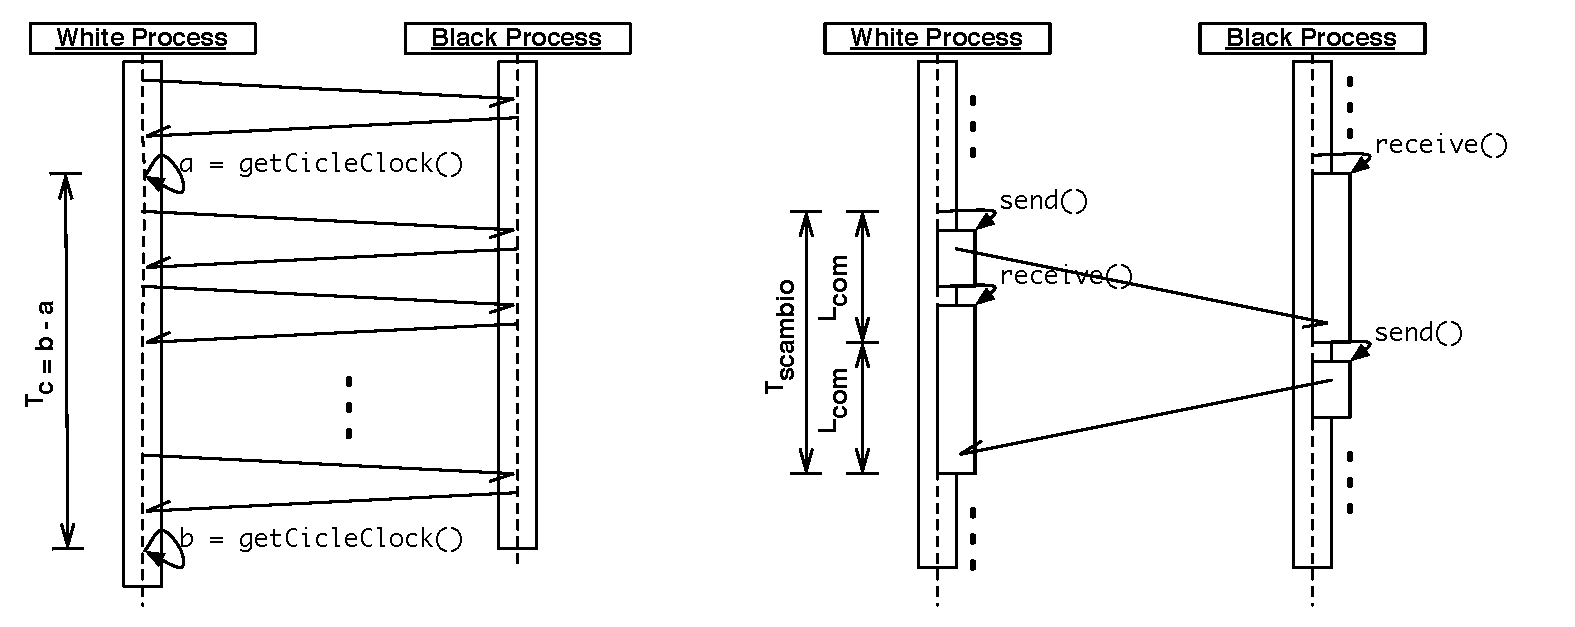
\includegraphics[scale=.5]{schema_metering.pdf}
  \caption[Comportamento temporale dell'applicazione ``ping-pong'']{Rappresentazione della sequenza di azioni svolte dai due processi dell'applicazione di misurazione. A sinistra viene mostrato il comportamento complessivo, a destra il dettaglio di uno scambio di messaggi.}
  \label{fig:schema_metering}
\end{figure}

Il programma di misurazione effettua $m$ scambi di messaggi. L'esecuzione e la corrispondente misurazione del tempo di completamento degli scambi \`e eseguita per diverse configurazioni di allocazione dei processi nei PE, a distanze diverse nella mesh. I valori di distanza, o \emph{numero di hops}, considerati sono: il minimo (1), il massimo (14) e quello medio ($\sqrt{64} = 8$). Per ogni configurazione vengono eseguite $n$ misure, ad ogni iterazione viene calcolato il valore medio della latenza di comunicazione per gli $m$ scambi effettuati. Per ogni distanza viene presentata la media, il valore massimo e la devianza standard degli $n$ valori medi della latenza di comunicazione. 

Nella misurazione della comunicazione asimmetrica si prendono in considerazione solo le due principali implementazioni del supporto, ovvero quella che fa uso della UDN e quella che utilizza al meglio la memoria condivisa \footnote{Per determinare questa informazione si usano i risultati della misura delle implementazioni simmetriche, si veda la discussione nella sezione~\ref{sct:meter_risultati}}. Inoltre, per la stessa forma di comunicazione e per quanto riguarda l'implementazione su memoria condivisa, viene fornita un'altra misura, chiamata \verb+ch_asymin_sm_all+. Viene utilizzato un canale asimmetrico con il massimo numero di processi mittenti allocabili nella macchina; come in precedenza, la misura \`e effettuata con lo scambio di messaggi tra due soli processi. La misura \`e interessante in quanto la politica di ricezione del destinatario prevede la scansione del flag \verb+Rdy+ di tutti i processi mittenti. \`E pertanto auspicabile un aumento della latenza di comunicazione con l'aumento del numero dei mittenti, anche se solo uno di questi comunica con il destinatario. Si osserva che questo secondo modo di misurare la comunicazione asimmetrica non fornisce risultati significati per l'implementazione UDN, e per questo motivo non \`e mostrato nei risultati. Con l'uso di UDN, infatti, la politica di ricezione non deterministica da pi\`u mittenti \`e implementata nativamente dal firmware della macchina e non \`e soggetta a overhead (\`e la lettura da una coda FIFO di registri).
